\documentclass[10pt,a4paper]{article}
\usepackage[utf8]{inputenc}
\usepackage{amsmath}
\usepackage{amsfonts}
\usepackage{amssymb}
\usepackage{graphicx}
\usepackage{caption}
\usepackage{subcaption}
\usepackage{float}
\usepackage{minted}
\usepackage{cite}
\usepackage[top=1.0in, bottom=1.0in, left=1.00in, right=1.00in]{geometry}

\usepackage{url}

\author{Chittaranjan Srinivas Swaminathan and Anders Wikström}
\title{Scortec ER-I Manipulator Control using Arduino Due}
\begin{document}
\maketitle
\tableofcontents
\newpage
\section{Introduction}
The Scortec ER-I is a 5-DOF manipulator from Eshed Robotec whose
control box is missing. The Manipulator consists of five
joints. Incremental optical encoders are mounted on the motor
shaft. Each encoder board consists of two Photodiode-LED pairs. This
enables us to measure both the angular displacement and the direction
of movement. The manipulator has a D50 connector connected to the
motors and the encoders.\\

The goal of this project is to use the Arduino
Due board and a motor shield to make a new controller for the
manipulator. 

Figure \ref{fig:axes} shows a sketch of the manipulator and the axes.

\begin{figure}[h]
    \centering
    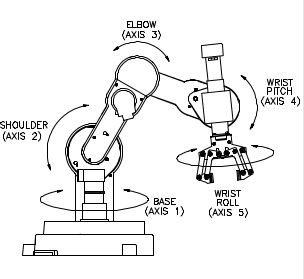
\includegraphics{axes.png}
    \caption{Scortec ER-I}
    \label{fig:axes}
\end{figure}

The task of creating a controller for the manipulator involves the
following steps:
\begin{enumerate}
\item Reverse engineer the motor and encoder connections and make a
  pinout diagram for the D50 connector on the manipulator.
\item Program the microcontroller to read the encoders.
\item Write control routines for position and velocity control.
\item Extend the control routines to more than one joint.
\end{enumerate}

The following sections describe each of these tasks and challenges
faced while executing them.

\section{Reverse Engineering}

In this task, we set out to map the pins on the D50 connector to the
individual motors and encoders. Once the pin-out diagram was in place
we could connect the Arduino and read the encoder pins. However, we
faced some problems while reading encoder outputs. The following
sections describe each of these tasks in detail. \\

\subsection{Pinout}
The primary task was to figure out the what each pin on the D50
connector meant. For this task we first took one motor and used the
multimeter to test for continuity. The process was repeated for each
motor and encoder board. Figuring out the circuit on the encoder board
was also important so as to understand which pins were the power
supply pins and which pins were the output pins.\\

The figure \ref{fig:dsub} is the pinout diagram. Note
that: \begin{itemize} 
\item \( E^a_b \) refers to output of encoder \textit{b} on joint \textit{a}.
\item \( GND^a \) refers to ground for encoder board on joint \textit{a}.
\item \( V^a_{cc} \) refers to power supply for encoder board on joint
\textit{a}.
\item \( M^a+ \) refers to the positive pin on motor \textit{a}.
\item \( M^a- \) refers to the negative pin on motor \textit{a}.
\end{itemize}


\begin{figure}[h]
    \centering
    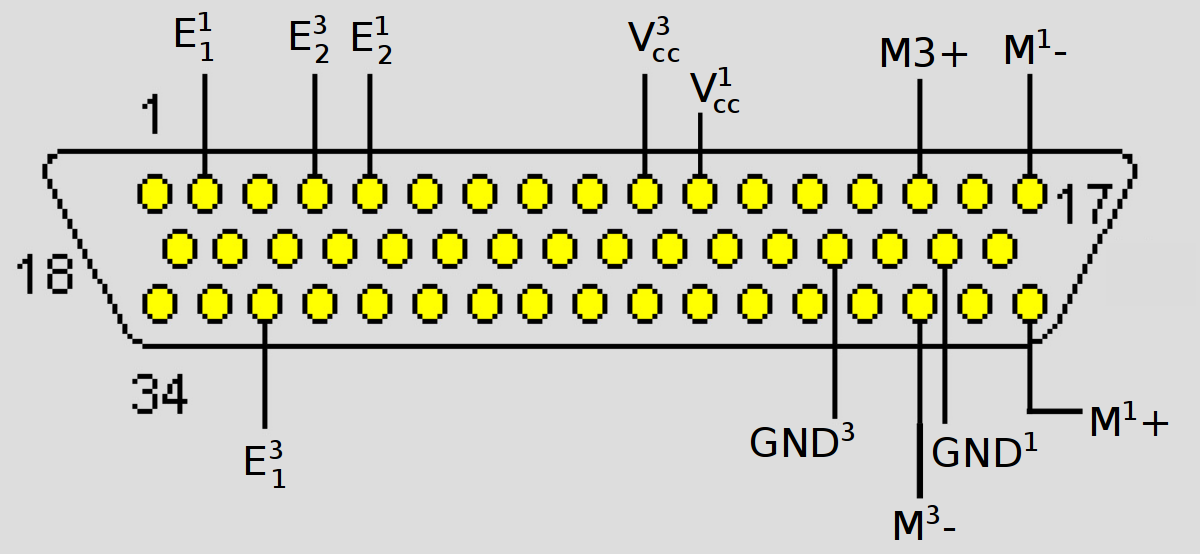
\includegraphics[scale=0.3]{dsub50.png}
    \caption{Pinout diagram for the D50 connector.}
    \label{fig:dsub}
\end{figure}

The motor has two pins (one positive and one negative) on the
connector. Each encoder board has a pair of encoders, thus enabling us
to read the incremental position of the joint as well as the direction
in which the joint is moving. The board has 6 pins but only 4 had
corresponding pins on the D50 connector. Also, it is important to
figure out what each of these pins meant.\\

To do this, we used the following steps:
\begin{enumerate}
\item The basic circuit for a Photodiode-LED pair is shown in figure
  \ref{fig:photodiodeLEDPair}. 
\item Detach the encoder board and use continuity test to figure out
  which components are connected.
\item Using the above two, figure out the circuit diagram of the
  board. This was found to be equivalent to the circuit in figure
  \ref{fig:encoderCircuit}. 
\item Finally, relate each pin on the encoder board to the
  circuit. 
\end{enumerate}

\begin{figure}[h]
    \centering
    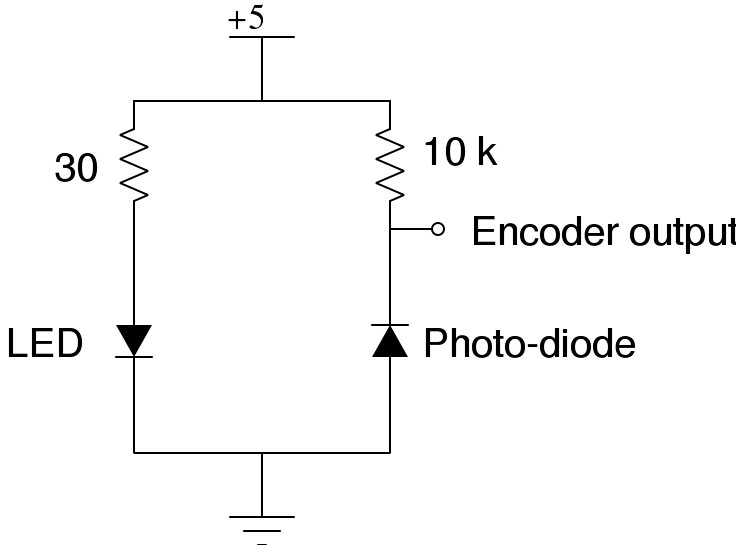
\includegraphics[scale=0.5]{SimpleEncoder.jpg}
    \caption{Basic circuit for Photodiode-LED pair.}
    \label{fig:photodiodeLEDPair}
\end{figure}

\begin{figure}[h]
    \centering
    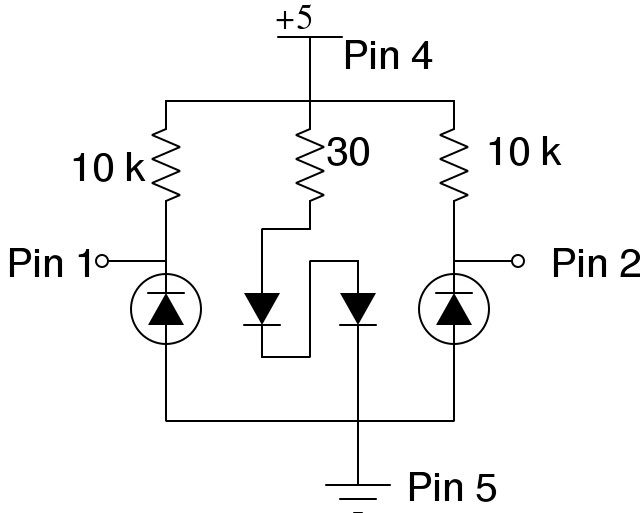
\includegraphics[scale=0.5]{EncoderCircuit.jpg}
    \caption{Equivalent Encoder circuit with two Photodiode-LED
      pairs. The photodiode is circled.}
    \label{fig:encoderCircuit}
\end{figure}

At this point, we were ready to read the encoder inputs from the
microcontroller. 

\subsection{Debouncing}

Routines to read the encoders were implemented from
\cite{ArduinoPlaygroundRE}.
The first test was to move the motor shaft by hand and check if the
rotation produced the necessary encoder ticks. This step gave positive
results. The next step was to move the joint by hand and see if the
incremental position was stable between motions. This step also gave
positive results. The position was only off by a few ticks every time
the joint was moved from one extremum position to another. \\

However, when the joint was moved using PWM input, we obtained far
more encoder ticks than when moved manually. Further inquiry lead us
to use a debouncer circuit shown in figure \ref{fig:rcfilter}. This is
also take from the Arduino Playground page on rotary encoders
\cite{ArduinoPlaygroundRE}.\\

\begin{figure}[h]
    \centering
    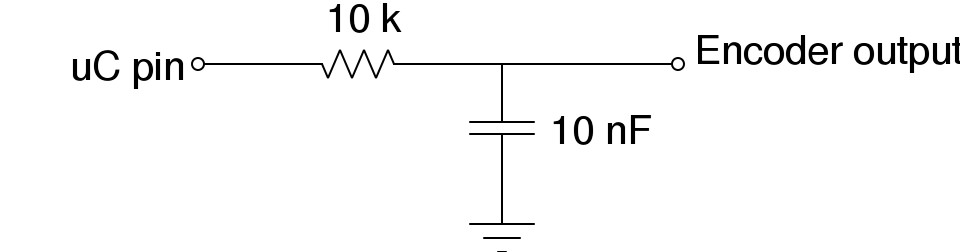
\includegraphics[scale=0.5]{debouncer.jpg}
    \caption{An RC filter for debouncing.}
    \label{fig:rcfilter}
\end{figure}

After introducing the RC Filter (hardware debounce circuit), the
encoder readings seemed to be fairly stable. Some errors were still
observed. 

\subsection{Current sensing}
We use current sensing to detect an extremum position, where the arm
is unable to move further. Since we use a PWM to control the motor, we
need some means of filtering the current so that we get a steadier
value than what we would get when we measure it directly. This is done
in two ways: 
\begin{enumerate}
\item A capacitor between the current pin and ground: the capacitor
  helps smooth out the current values.
\item A software low-pass filter.
\end{enumerate}

\section{Control routines}

In this section, the control routines and organization of code is
described. We employ a PID controller for velocity 

\subsection{Calibration}

The main aim of calibration is to find out how many pulses are
received for every degree that the joint moves. The range of the each
joint was taken from the datasheet of the manipulator. Then, we
calculated the total encoder ticks for the full range of a joint. We
then computed a ratio to convert angular displacement/velocity
described in encoder ticks to degrees. That is,
\[ \alpha = \frac{range\ of\ joint}{measured\ encoder\ ticks}\]

where \(\alpha\) is the ratio described above\footnote{The ratio
  \(\alpha\) is simply called 'ratio' in code.}. The unit of
\(\alpha\) is \( \frac{encoder\ ticks}{degree}\). \\


Each joint is calibrated as follows:
\begin{itemize}
\item The joint to be calibrated is first moved in the negative
  direction\footnote{Negative direction is the direction that results
    in negative encoder readings} till the extremum is reached. The
  extremum point is detected by measuring the current.
\item At this point the encoder value is reset. 
\item The joint is then moved to the other extremum in the positive
  direction, at which point calibration ends.
\item The encoder value at positive extremum is the total encoder
  ticks for full range movement of the joint.
\end{itemize}

\subsubsection{Results from calibration}

We observed that the number of ticks over the full range varied more
than a few tens of ticks. Hence, we averaged the measured ticks and
computed a ratio from the average. \\ 

\begin{tabular}{ | l | r | r |}
\hline
- & \textbf{Joint 1} & \textbf{Joint 3} \\
\hline
1 & 9748 & 3195 \\
\hline
2 & 9924 & 3178 \\
\hline
3 & 9832 & 3181 \\
\hline
4 & 9850 & 3193 \\
\hline
5 & 9796 & 3194 \\
\hline
\textbf{Mean} & 9830 & 3188.2 \\
\hline
\textbf{Ratio} & 30.71875 & 17.049 \\
\hline

\end{tabular}

\subsection{Position Control}
The position controller looks at the direction the arm have to move to reach the desired position. When is given a new position command is given, position control activates velocity control with a set velocity. Position control continuously check is the correct position has been reached and stops the velocity control.

\subsection{Velocity Control}
The velocity of the joints are controlled by a PID controller. The controller tries to move at a constant velocity in the direction given by the position control. 

\subsection{Overall organization of code}
Each joint is controlled by an independent motor controller that contains all information needed to control its joint. The motor controller stores things such as PIN numbers for encoders, current sensing and stores state information used for the encoders and PID controllers.

\section{Evaluation of the system}
Two methods:
\begin{itemize}
\item Accuracy and precision of the incremental optical encoders.
\item Accuracy and precision of the control system.
\end{itemize}

\subsection{Accuracy and Precision for Joint 1}
To evaluate the performance of our controller we did some tests. The most important aspects of performance for the controller would be its accuracy and precision. \\

We decided to run the test on Joint 1 since it is not affected by gravity in the axis of rotation. First we marked two locations on the base of the robot we measured to be 90 degrees away from each other.  We ran our test by moving Joint one from one of the points, record the angle our controller reported, then moved it back and recorded that angle. The circumference of the base of the joint was measured to be 66.8 cm and angles were measured by measuring arc lengths. The least count of the tape used is 0.1 cm. This gives us a least count of 0.54 degrees.\\

%\begin{tabular}{ | l | r |}
%\hline
%\textbf{Joint 1} & \textbf{Error} \\
%\hline
% 165.10 &  \\
%\hline
% 251.79 & 3.31 \\
%\hline
% 167.31 & 5.52 \\
%\hline
% 251.72 & 5.59 \\
%\hline
% 168.00 & 6.28\\
%\hline
% 254.58 & 3.42\\
%\hline
%167.90 & 3.32\\
%\hline
%253.93 & 3.97\\
%\hline
%168.10 & 4.17\\
%\hline
%252.76 & 5.34\\
%\hline
%168.13 & 5.37\\
%\hline
%\end{tabular} \\

\begin{tabular}{ | l | r |}
\hline
\textbf{Measured} & \textbf{Error} \\
\hline
 86.69 & 3.31 \\
\hline
 84.48 & 5.52 \\
\hline
 84.41 & 5.59 \\
\hline
 83.72 & 6.28 \\
\hline
 86.58 & 3.42\\
\hline
 86.68 & 3.32\\
\hline
86.03 & 3.97\\
\hline
85.83 & 4.17\\
\hline
84.66 & 5.34\\
\hline
84.63 & 5.37\\
\hline
\end{tabular} \\ 

%\hline
%\textbf{Mean error} & \textbf{Variance}\\
%\hline
% 4.63 & 1.23 \\
%\hline
%5.14\%  &  \\
%\hline
%\end{tabular}

The mean error in this test is 4.63 degrees and that becomes an error of 5.14\%. Thus without further signal possessing and filtering the accuracy of the encoder probably not good enough for any real use case. The precision is better, the variance is 1.23.\\

We repeated the experiment but instead of moving Joint 1 by hand we moved it with our controller. We made the controller move at approximately the same speed as when we move the joint by hand. The table below shows commands when we told it to move 30 degrees, the sensed value is the value the controller reports when it stops. \\

\begin{tabular}{ | l | r | r |}
\hline
\textbf{Measured} & \textbf{Sensed} & \textbf{Error} \\
\hline
 28.02 & 28.58 & 0.56  \\
\hline
 28.56	& 28.78 & 0.21 \\
\hline
 28.56 & 28.91 & 0.35 \\
\hline
 29.10 & 28.74 & 0.36 \\
\hline
 29.64 & 28.94 & 0.70\\
\hline
\end{tabular} \\

We can see that the mean error is 0.43 or 1.45\% with a variance of 0.27. The std and the mean is comparable to the least count of the measurement used.
As we can see the error in position measurement is less than when we moved the joint by hand. We suspect this is caused by a systematic error present when moving the joints with our controller and since we do the calibration with the motors powered, the systematic error is canceled.

\section{Future Work}

The following summarizes some of the possible future work that can be
done with the manipulator: 

\begin{itemize}
\item After obtaining ratios for each joint from calibration, we could
  replace the calibration routines with ``home'' routine. When the arm
  is HOME-d, each joint simply moves to the negative extremum
  position. 
\item Add all joints. Framework is ready.
\item Do some forward kinematics and output tf to ROS.
\end{itemize}

\bibliographystyle{ieeetr}
\bibliography{report}

\end{document}